\begin{name}
{\tenchude}{\tendethi}{LỚP TOÁN THẦY PHÁT}{\thoigian}
\end{name}

\Opensolutionfile{ans}[ans/ansBTTeX1]

\begin{ex}%[2D3B1-2]%
Nguyên hàm $\displaystyle \int \dfrac{1+\ln x}{x} \mathrm{\, d}x$ $(x>0)$ bằng
\choice
{\True $\dfrac{1}{2}\ln^2x + \ln x + C$ }
{ $x+\dfrac{1}{2}\ln^2x + C$}
{ $\ln^2x + \ln x + C$}
{ $x+\ln^2x + C$}
\loigiai{
Xét $I=\displaystyle \int \dfrac{1+\ln x}{x} \mathrm{\, d}x$\\
Đặt $t = \ln x \Rightarrow \mathrm{\, d}t=\dfrac{1}{x}\mathrm{\, d}x$. Ta được \\
$I =\displaystyle \int (1+t) \mathrm{\, d}t = t+\dfrac{t^2}{2} +C= \ln x + \dfrac{1}{2} \ln^2 x+C $.
}
\end{ex}

\begin{ex}%[2D3K2-3]%
Cho tích phân $I=\displaystyle \int\limits_{1}^{\mathrm{e}}\left(x+1\right)\ln x \mathrm{d}x=\dfrac{\mathrm{e}^2+a}{b}$ với $a,b$ là những số nguyên dương. Giá trị của biểu thức $T=a+b$ tương ứng bằng
\choice
{$8$}
{$10$}
{$7$}
{\True $9$}
\loigiai{
Đây là tích phân từng phần. Đặt $\heva{
&u=\ln x \\ &\mathrm{d}v = \left(x+1\right)\mathrm{d}x
} \Rightarrow \heva{
&\mathrm{d}u = \dfrac{\mathrm{d}x}{x}\\ &v =\dfrac{x^2+2x}{2}}.$\\
Suy ra $I=\displaystyle \int\limits_{1}^{e}\left(x+1\right)\ln x \mathrm{d}x = \dfrac{x^2+2x}{2} \ln x \bigg|_1^{\mathrm{e}}-\int\limits_{1}^{\mathrm{e}}\dfrac{x^2+2x}{2}\cdot \dfrac{\mathrm{d}x}{x}=\dfrac{\mathrm{e}^2+2\mathrm{e}}{2}-\int_{1}^{\mathrm{e}}\dfrac{x+2}{2}\mathrm{d}x$.\\
Dẫn đến $I=\dfrac{\mathrm{e}^2+5}{4}=\dfrac{\mathrm{e}^2+a}{b}$.\\
Suy ra $\heva{
&a=5 \\&b=4.}$
\\ $T=a+b=4+5=9$.
}
\end{ex}

\begin{ex}%[Tổng ôn LVD-GV soạn Mui Doan-GVPB Khanh Lê]%[2D3B2-3]%
Cho hàm số $ f(x) $ có $ f(0)= 0 $ và  $ f'(x)=x\sin x, \forall x\in\mathbb{R} $. Khi đó $ \displaystyle\int\limits_0^{\frac{\pi}{2}} f(x)\mathrm{\,d}x $ bằng
\choice
{$ -1 $}
{$ \dfrac{1}{2} $}
{\True $ 2-\dfrac{\pi}{2} $}
{$ 1 $}
\loigiai{
Vì $ f'(x)=x\sin x$ nên	$ f(x)= \displaystyle\int x\sin x\mathrm{\,d}x  $.\\
Đặt $ \heva{&u=x\\&\mathrm{\,d}v=\sin x\mathrm{\,d}x}\Rightarrow\heva{&\mathrm{\,d}u=\mathrm{\,d}x\\&v=-\cos x} $
\begin{eqnarray*}
\Rightarrow f(x)&=&-x\cos x-\displaystyle\int -\cos x\mathrm{\,d}x\\
&=&-x\cos x+\sin x+C.
\end{eqnarray*}
Do $ f(0)=0\Rightarrow C=0$.\\
Vậy $ f(x)=-x\cos x+\sin x$.
Ta có
\allowdisplaybreaks
\begin{eqnarray*}
\displaystyle\int\limits_0^{\frac{\pi}{2}} f(x)\mathrm{\,d}x
&=&\displaystyle\int\limits_0^{\frac{\pi}{2}} \left(-x\cos x+\sin x\right)\mathrm{\,d}x\\
&=& \displaystyle\int\limits_0^{\frac{\pi}{2}} -x\mathrm{\,d}(\sin x)+\displaystyle\int\limits_0^{\frac{\pi}{2}} \sin x\mathrm{\,d}x \\
&=&-x\sin x\bigg|^{\frac{\pi}{2}}_0+\displaystyle\int\limits_0^{\frac{\pi}{2}} \sin x\mathrm{\,d}x+\displaystyle\int\limits_0^{\frac{\pi}{2}} \sin x\mathrm{\,d}x\\
&=&-\dfrac{\pi}{2}-2\cos x\bigg|^{\frac{\pi}{2}}_0\\
&=&-\dfrac{\pi}{2}-0+2\\
&=&2-\dfrac{\pi}{2}.
\end{eqnarray*}
}
\end{ex}

\begin{ex}%[2H3B2-3]%
Trong không gian $Oxyz$, cho hai điểm $A(2;1;0)$ và $B(0;-1;4)$. Mặt phẳng trung trực của đoạn thẳng $AB$ có phương trình là
\choice
{$2x+y-2=0$}
{$2x+y+z-4=0$}
{\True $x+y-2z+3=0$}
{$-x-y+2z+3=0$}
\loigiai
{
Gọi $M$ là trung điểm của $AB\Rightarrow M(1;0;2)$.\\
Mặt phẳng trung trực của đoạn thẳng $AB$ có một vectơ pháp tuyến là $\overrightarrow{AB}=(-2;-2;4)$.\\
Mặt phẳng trung trực của $AB$ đi qua $M(1;0;2)$ và nhận $\overrightarrow{AB}$ làm vectơ pháp tuyến nên phương trình mặt phẳng là $$-2(x-1)-2y+4(z-2)=0\Leftrightarrow -x-y+2z-3=0\Leftrightarrow x+y-2z+3=0.$$
}
\end{ex}

\begin{ex}%[2D3B2-3]%Câu 467.
Nếu $\displaystyle\int_1^a\ln x \mathrm{\, d}x=1+2 a$ với $a>1$ thì $a$ thuộc khoảng nào sau đây?
\choice
{\True $(18; 21)$}
{$(1; 4)$}
{$(11; 14)$}
{$(6; 9)$}
\loigiai{
Đặt $\heva{& u=\ln x\Rightarrow \mathrm{\,d}u=\dfrac{1}{x}\mathrm{\,d}x \\ & \mathrm{\,d}v= \mathrm{\,d}x\Rightarrow v=x.}$\\
Khi đó $\displaystyle\int_1^a\ln x \mathrm{\,d}x=x\cdot\ln x\bigg|_1^a-\displaystyle\int_1^a x\cdot\dfrac{1}{x} \mathrm{\,d}x=a\ln a-x\bigg|_1^a=a\ln a-a+1$.\\
Theo giả thiết, ta có $a\ln a-a+1=1+2a\Leftrightarrow \ln a=3\Leftrightarrow a=\mathrm{e}^3\in(18;21)$.
}
\end{ex}

\begin{ex}%[Phạm Hoàng Điệp]%[2H3K2-3]%
Trong không gian $Oxyz$, biết mặt phẳng $ax+by+cz-24=0$ qua $A(1;2;3)$ và vuông góc với hai mặt phẳng $(P)\colon 3x-2y+z+4=0$, $(Q)\colon 5x-4y+3z+1=0$. Giá trị $a+b+c$ bằng
\choice
{$ 8 $}
{$ 9 $}
{$ 10 $}
{\True $ 12 $}
\loigiai{
Gọi $ \alpha $ là mặt phẳng cần tìm và $ \overrightarrow{n}_{(\alpha)} $ là một véc-tơ pháp tuyến của mặt phẳng $ \alpha $.\\
Mặt phẳng $ (P)\colon 3x-2y+z+4 =0$ có véc-tơ pháp tuyến $ \overrightarrow{n}_{P}(3;-2;1) $, mặt phẳng $ (Q) $ có véc-tơ pháp tuyến $ \overrightarrow{n}_{Q}(5;-4;-2) $.\\
Ta có $ \heva{&(\alpha)\perp (P)\\&(\alpha)\perp (Q)} \Rightarrow\overrightarrow{n}_{(\alpha)} =\left[\overrightarrow{n}_{P}.\overrightarrow{n}_{Q}\right]=(-2;-4;-2)$.\\
Mặt phẳng $ (\alpha) $ qua $ A $ có véc-tơ pháp tuyến $ \overrightarrow{n}_{(\alpha)} $ có phương trình là\\
$ -2(x-1)-4(y-2)-2(z-3)=0 \Leftrightarrow -2x-4y-2z+16=0\Leftrightarrow (\alpha)\colon 3x+6y+3z=0$.\\
Vậy $ a+b+c=3+6+3=12 $.
}
\end{ex}

\begin{ex}%[Dat Thai, Dự án Tư Duy Mở]%[2D3Y3-1]%
\immini
{
Cho hình phẳng $(H)$ giới hạn bởi các đường $y=f(x)$, $y=g(x)$, $y=h(x)$ có đồ thị biểu diễn như hình vẽ. Diện tích hình phẳng giới hạn bởi hình $(H)$ tính theo công thức
}
{
\begin{tikzpicture}[line join=round, line cap = round, >=stealth, scale=.8,font=\footnotesize,transform shape]
\foreach \x/\y/\z/\g in
{
1/0/1/-90,4/0/4/-90,7/0/7/-90,
0/0/O/-135
}
\draw[fill=black] (\x,\y) circle(1pt) coordinate (\z) ($(\z)+(\g:3mm)$) node{$\z$};
\draw[samples=100,domain=-.5:5.5] plot(\x,{((\x)^2+2*\x +18)/21}) node[right]{$f(x)$};
\draw[samples=100,domain=7.5:3] plot(\x,{((\x)^2-16*\x +78)/15}) node[above]{$g(x)$};
\draw[samples=100,domain=-.5:7.5] plot(\x,{((\x)^2-8*\x +25)/18}) node[above]{$h(x)$};
\draw[draw=none, pattern = dots, pattern color=black!80, samples=100] plot[domain=1:4](\x,{((\x)^2+2*\x +18)/21})--plot[domain=4:7](\x,{((\x)^2-16*\x +78)/15})--plot[domain=7:1](\x,{((\x)^2-8*\x +25)/18})--cycle;
\draw[->] (-1,0)--(8,0) node[below]{$x$};
\draw[->] (0,-1)--(0,3) node[right]{$y$};
\draw[dashed] (1,0)--(1,1) (4,0)--(4,2) (7,0)--(7,1);
\end{tikzpicture}
}
\choice
{$S = \displaystyle\int\limits_1^4 \left[ f(x) - h(x) \right] \mathrm{\,d}x + \displaystyle\int\limits_4^7 \left[ h(x) - g(x) \right] \mathrm{\,d}x$}
{$S = \displaystyle\int\limits_1^4 \left[ f(x) - g(x) \right] \mathrm{\,d}x + \displaystyle\int\limits_4^7 \left[ g(x) - h(x) \right] \mathrm{\,d}x$}
{$S = \displaystyle\int\limits_1^4 \left[ h(x) - g(x) \right] \mathrm{\,d}x + \displaystyle\int\limits_4^7 \left[ f(x) - g(x) \right] \mathrm{\,d}x$}
{\True $S = \displaystyle\int\limits_1^4 \left[ f(x) - h(x) \right] \mathrm{\,d}x + \displaystyle\int\limits_4^7 \left[ g(x) - h(x) \right] \mathrm{\,d}x$}
\loigiai{
Nhìn vào hình vẽ ta thấy
\begin{itemize}
\item $f(x) \ge h(x)$ với mọi $x\in(1;4)$;
\item $g(x) \ge h(x)$ với mọi $x\in(4;7)$.
\end{itemize}
Do đó diện tích hình phẳng $(H)$ là
\[
S = \displaystyle\int\limits_1^4 \left[ f(x) - h(x) \right] \mathrm{\,d}x + \displaystyle\int\limits_4^7 \left[ g(x) - h(x) \right] \mathrm{\,d}x.
\]
}
\end{ex}

\begin{ex}%[2D4G5-1]%
Cho số phức $ z $ thỏa mãn $ |z-2-3i|+|z+1+i|=5 $. Gọi giá trị lớn nhất và giá trị nhỏ nhất của biểu thức $ T=|z-2| $ tương ứng là $ a $ và $ b $. Giá trị biểu thức $ T=a+b $ bằng
\choice
{\True $ \sqrt{10}+\dfrac{9}{5} $}
{$ \sqrt{13}+\sqrt{3} $}
{$ 1+\sqrt{5} $}
{$ 2+\sqrt{10} $}
\loigiai{
Ta gọi điểm $M$ biểu diễn số phức $z$ và điểm $A(2 ; 3), B(-1 ; -1)\Rightarrow AB=5$.\\
Suy ra  $|z-2-3i|+|z+1+i|=5\Leftrightarrow MA+MB=AB$.\\
Suy ra $M$ nằm trên đoạn thẳng $AB$.\\
Hình vẽ minh họa
\begin{center}
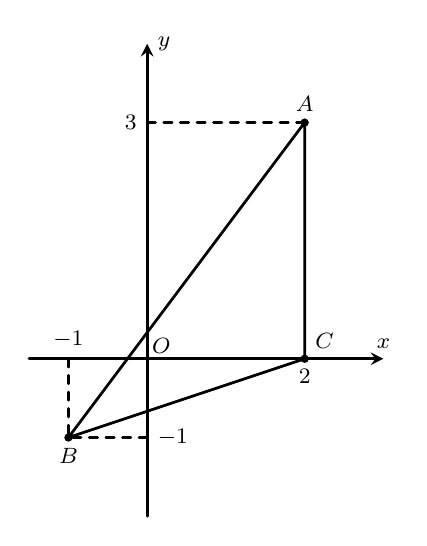
\begin{tikzpicture}[>=stealth,line join=round,line cap=round,line width=1pt,font=\footnotesize]
\draw[->](-1.5,0)--(0,0)node [above right=-2pt]{$ O $}--(3,0) node [above]{$ x $};
\draw[->](0,-2)--(0,4)node [right]{$ y $};
\coordinate[label=above:$A$](A) at (2,3);
\coordinate[label=below:$B$](B) at (-1,-1);
\coordinate[label=above right:$C$](C) at (2,0);
\foreach \toado in {(A),(B),(C)}
{
\fill \toado  circle (1.5 pt);
}
\draw (A)--(B)--(C)--(A);
\draw [dashed] (-1,0)node [above]{$ -1 $}--(B)--(0,-1)node [right]{$ -1 $};
\draw[dashed](0,3)node [left]{$ 3 $}--(A);
\node [below] at (2,0){$ 2 $};
\end{tikzpicture}
\end{center}
Gọi điểm $ C(2 ; 0) $. Suy ra, biểu thức $ T=|z-2|=MC $ (với $ M $ nằm trên đoạn $ AB$).\\
Ta có $ CA=3 $, $ CB=\sqrt{10} $.\\
Suy ra giá trị lớn nhất của biểu thức $ T $ là $ T_{max}=CM_{max}=CB=\sqrt{10}=a $ khi $ M \equiv B $.\\
Biểu thức $T$ đạt giá trị nhỏ nhất là $T_{\min } = CM_{\min }= CH$; với $H$ là hình chiếu vuông góc của điểm $C$ lên đoạn thẳng $AB$.\\
Dễ dàng tìm được đường thẳng $(AB): 4x-3y+1=0$.\\
Suy ra $ CH=d\left(C, AB \right)=\dfrac{9}{5} \Rightarrow T_{min}=CH=\dfrac{9}{5}=b$.\\
Suy ra $ a+b=\sqrt{10}+\dfrac{9}{5} $.
}
\end{ex}

\begin{ex}%[Dự án Texbook 12 -quyển 3]%[Phan Văn Thành]%[2H3K3-7]%
Trong không gian với hệ tọa độ $Oxyz$, cho mặt phẳng $\left( P \right)\colon x+y-z-3=0$ và hai điểm $M\left( 1;1;1 \right)$, $N\left( -3;-3;-3 \right)$. Mặt cầu $(S)$ đi qua hai điểm $M$, $N$ và tiếp xúc với mặt phẳng $(P)$ tại điểm $Q$. Biết rằng $Q$ luôn thuộc một đường tròn cố định. Tính bán kính $R$ của đường tròn đó.
\choice
{ $R=\dfrac{2\sqrt{11}}{3}$}
{ $R=\dfrac{2\sqrt{33}}{3}$}
{\True $R=6$}
{ $R=4$}
\loigiai{
Phương trình đường thẳng $MN\colon \dfrac{x-1}{1}=\dfrac{y-1}{1}=\dfrac{z-1}{1}$.\\
Gọi $\{E\}=MN\cap (P)$. Suy ra tọa độ điểm $E$ thỏa hệ
$$\heva{& \dfrac{x-1}{1}=\dfrac{y-1}{1}=\dfrac{z-1}{1}\\& x+y-z-3=0}\Leftrightarrow \heva{& x=3\\& y=3\\& z=3}\Rightarrow E(3;3;3).$$
Suy ra $EM=2\sqrt{3}$; $EN=6\sqrt{3}$.\\
Ta có $\triangle EQM$ và $\triangle ENQ$ đồng dạng, suy ra $\dfrac{EQ}{EN}=\dfrac{EM}{EQ}\Rightarrow EQ^2=EM \cdot EN=36$.\\
Vậy $EQ=6$. Do đó điểm $Q$ thuộc đường tròn tâm $E$, bán kính $R=6$.
}
\end{ex}

\begin{ex}%[2D3Y3-1]%Câu 497.
\immini[thm]
{
Diện tích phần hình phẳng gạch chéo trong hình vẽ được tính theo công thức nào dưói đây?
\choice
{\True $\displaystyle\int_{-1}^0(2x^3-2x) \mathrm{\,d}x+\displaystyle\int_0^1(2x-2x^3) \mathrm{\,d}x$}
{$\displaystyle\int_{-1}^1(2x^3-2x) \mathrm{\,d}x$}
{$\displaystyle\int_{-1}^1(2x-2x^3) \mathrm{\,d}x$}
{$\displaystyle\int_{-1}^0(2x^3-2x) \mathrm{\,d}x-\displaystyle\int_0^1(2x-2x^3) \mathrm{\,d}x$}
}
{
\begin{tikzpicture}[scale=1,font=\footnotesize,line join = round, line cap = round,>=stealth,x=1cm,y=0.7cm]
\def\hsf(#1){-2*(#1)^3+(#1)^2+(#1)+3}
\def\hsg(#1){(#1)^2-(#1)+3}
\draw[->] (-1.2,0)--(0,0)node[below left]{$O$}--(2,0)node[below]{$x$};
\draw[->] (0,-1)--(0,5.5)node[left]{$y$};
\draw[samples=100,domain=-1.08:1.39,smooth] plot (\x, {\hsf(\x)});
\draw[samples=100,domain=-1.17:1.61,smooth] plot (\x, {\hsg(\x)});
\draw[pattern = north east lines,opacity=0.5,draw=none] plot[domain=-1:1] (\x, {\hsf(\x)})--plot[domain=1:-1] (\x, {\hsg(\x)})--cycle;
\draw[dashed,thin] (-1,{\hsg(-1)})--(-1,0)node[below]{$-1$} (1,{\hsg(1)})--(1,0)node[below]{$1$};
\path (1.2,2.5)node[right,rotate=60]{$y=x^2-x+3$} (1.4,1)node[right,rotate=60]{$y=-2x^3+x^2+x+3$};
\end{tikzpicture}
}
\loigiai{
Từ hình vẽ ta có diện tích là $\displaystyle\int_{-1}^0(2x^3-2x) \mathrm{\,d}x+\displaystyle\int_0^1(2x-2x^3) \mathrm{\,d}x$.
}
\end{ex}

\begin{ex}%[2H3B1-3]%
Tìm độ dài đường kính của mặt cầu $(S)$ có phương trình $x^2+y^2+z^2-2y+4z+2=0$.
\choice
{$\sqrt{3}$}
{$2$}
{$1$}
{\True $2\sqrt{3}$}
\loigiai{
Bán kính của mặt cầu $R=\sqrt{1^2+(-2)^2-2}=\sqrt{3}\Rightarrow $ đường kính của mặt cầu là $2R=2\sqrt{3}$.
}
\end{ex}

\begin{ex}%[2H3B2-3]%
Trong không gian $O x y z$, phương trình mặt phẳng đi qua $M(3 ;-1 ; 2)$, $N(4 ;-1 ;-1)$, $P(2 ; 0 ; 2)$ là
\choice
{$3 x+3 y-z+8=0$}
{$3 x-2 y+z-8=0$}
{\True $3 x+3 y+z-8=0$}
{$3 x+3 y-z-8=0$}
\loigiai{
Ta có $\overrightarrow{MN}=(1;0;-3)$, $\overrightarrow{MP}=(-1;1;0)$.\\
Mặt phẳng đi qua điểm $M(3 ;-1 ; 2)$ và có véc-tơ pháp tuyến $\vec{n}=\left[\overrightarrow{MN},\overrightarrow{MP}\right]=(3;3;1)$ có phương trình là
$$3(x-3)+3(y+1)+1(z-2)=0\Leftrightarrow 3x+3y+z-8=0.$$
}
\end{ex}

\begin{ex}%[2D3Y3-3]%
Hình $ (H) $  giới hạn bởi các đường  $ y=f(x) $,  $ x=a $, $ x=b \,(a<b)$    và trục  $ Ox $. Khi quay $ (H) $  quanh trục $ Ox $  ta được một khối tròn xoay có thể tích tính bằng công thức sau
\choice
{$ V=\pi \displaystyle\int\limits_a^b\vert f(x)\vert\mathrm{\,d}x $}
{$ V=\pi \displaystyle\int\limits_a^b f(x)\mathrm{\,d}x $}
{\True $ V=\pi \displaystyle\int\limits_a^b f^2(x)\mathrm{\,d}x $}
{$ V= \displaystyle\int\limits_a^b f(x)\mathrm{\,d}x $}
\loigiai{
Ta có 	$ V=\pi \displaystyle\int\limits_a^b f^2(x)\mathrm{\,d}x $.
}
\end{ex}

\begin{ex}%[2D3Y2-1]%
Cho hàm số $F(x)$ là một nguyên hàm của hàm số $f(x)$ trên đoạn $[a;b]$. Tích phân $\displaystyle\int\limits_a^b f(x)\mathrm{d}x$ bằng
\choice
{\True $F(b)-F(a)$}
{$F(a)-F(b)$}
{$f(b)-f(a)$}
{$f(a)-f(b)$}
\loigiai{
Theo giả thiết $F(x)$ là một nguyên hàm của hàm số $y=f(x)$ trên đoạn $[a;b]$ nên ta có $$\displaystyle\int\limits_a^bf(x)\mathrm{d}x=F(x)\Big|^{b}_{a}=F(b)-F(a).$$
}
\end{ex}

\begin{ex}%[2D4Y1-1]%
Cho số phức $z=5+3i$. Số phức liên hợp của $z$ là
\choice
{$-5+3i$}
{$-5-3i$}
{\True $5-3i$}
{$5i-3$}
\loigiai{
Số phức $z=a+bi$ $\left(a;b\in \mathbb{R}\right)$ có số phức liên hợp là $\overline{z}=a-bi$.\\
Vậy số phức $z=5+3i$ có số phức liên hợp là $\overline{z}=5-3i$.
}
\end{ex}

\begin{ex}%[2D3Y1-1]%Câu 24
$\displaystyle\int\limits 5x^4 \mathrm{\,d}x$ bằng
\choice
{$20x^3+C$}
{$\dfrac{1}{5}x^5+C$}
{$5x^5+C$}
{\True $x^5+C$}
\loigiai{
$\displaystyle\int\limits 5x^4 \mathrm{\,d}x=x^5+C$.}
\end{ex}

\begin{ex}%[2D4B3-2]%
Cho hai số phức $z_1$, $z_2$ thỏa mãn điều kiện $z_1+(2+3i)z_2=1-3i$; $(1-i)z_1+(1+i)z_2=2$. Giá trị của biểu thức $T=\left|z_1+iz_2\right|$ bằng
\choice
{$\sqrt{2}$}
{$\sqrt{3}$}
{\True $2$}
{$1$}
\loigiai{
Từ giả thiết ta có $\heva{&z_1+(2+3i)z_2=1-3i\\&(1-i)z_1+(1+i)z_2=2} \Rightarrow z_2\left[(2+3i)-i\right]=1-3i-(1+i)$\\
$\Leftrightarrow z_2=\dfrac{-4i}{2+2i}=-1-i$.\\
Thế $z_2$ vào hệ ta được $z_1=2i$.\\
Suy ra $T=\left|z_1+iz_2\right|=\left|2i+i(-1-i)\right|=\sqrt{2}$.
}
\end{ex}

\begin{ex}Câu 35%[2D4Y3-1]%
Cho số phức $z$ thỏa mãn $iz=5+4i$. Số phức liên hợp của $z$ là
\choice
{\True $\overline{z}=4+5i$}
{$\overline{z}=4-5i$}
{$\overline{z}=-4+5i$}
{$\overline{z}=-4-5i$}
\loigiai{
Ta có $iz=5+4i$ $\Rightarrow z=\dfrac{5+4i}{i} \Rightarrow z=4-5i$ $\Rightarrow \overline{z}=4+5i$.
}
\end{ex}

\begin{ex}%[TDM21]%[Võ Thị Thùy Trang]%[2H3Y3-3]%
Trong không gian với hệ tọa độ $Oxyz$, cho đường thẳng $d\colon \dfrac{x-1}{2}=\dfrac{y-2}{-1}=\dfrac{z}{2}$. Điểm nào dưới đây không thuộc đường thẳng $d$?
\choice
{\True $\left(3;1;-2\right)$}
{$\left(1;2;0\right)$}
{$\left(-1;3;-2\right)$}
{$\left(3;1;2\right)$}
\loigiai{
Do $ \dfrac{3-1}{2}=\dfrac{1-2}{-1}\ne\dfrac{-2}{2}$ nên điểm $\left(3;1;-2\right)$ không thuộc đường thẳng $d$.
}
\end{ex}

\begin{ex}%[Hình học Oxyz, Tư duy mở]%[Lê Hồng Phi]%[2H3Y3-6]%
Trong không gian tọa độ $Oxyz$, cho hai đường thẳng $\Delta_1\colon \dfrac{x-1}{5}=\dfrac{y-3}{-2}=\dfrac{z+3}{1}$ và đường thẳng $\Delta_2\colon \dfrac{x-3}{-5}=\dfrac{y+1}{2}=\dfrac{z-1}{-1}$. Nhận xét đúng về vị trí tương đối của hai đường thẳng $\Delta_1$, $\Delta_2$ là
\choice
{\True $\Delta_1\parallel\Delta_2$}
{$\Delta_1$ cắt $\Delta_2$}
{$\Delta_1\equiv\Delta_2$}
{$\Delta_1$ chéo $\Delta_2$}
\loigiai{
Đường thẳng $\Delta_1$, $\Delta_2$ lần lượt có véc-tơ chỉ phương là $\overrightarrow{u}_1=(5;-2;1)$ và $\overrightarrow{u}_2=(-5;2;-1)$.\\
Vì $\overrightarrow{u}_1=-\overrightarrow{u}_2$ nên $\Delta_1\parallel\Delta_2$ hoặc $\Delta_1\equiv\Delta_2$.\\
Ta có $M(1;3;-3)\in\Delta_1$ nhưng $M\notin\Delta_2$ nên $\Delta_1\parallel\Delta_2$.
}
\end{ex}

\begin{ex}%[2D4B1-2]%
\immini{
Trong mặt phẳng phức, cho $z=1+i$ điểm nào dưới đây biểu diễn đúng số phức $iz$?
\choice
{\True Điểm $A$}
{Điểm $B$}
{Điểm $C$}
{Điểm $D$}
}{
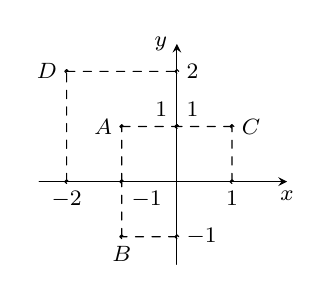
\begin{tikzpicture}[scale=.7,font=\footnotesize,line cap=round,line join=round,>=stealth]
\draw[->] (-2.5,0)--(2,0)node[below]{$x$};
\draw[->] (0,-1.5)--(0,2.5)node[left]{$y$};
\draw[dashed] (-1,0)node[below right]{$-1$}circle(1pt)--(-1,1)node[left]{$A$}circle(1pt)--(0,1)node[above left]{$1$}circle(1pt);
\draw[dashed] (0,-1)node[right]{$-1$}circle(1pt)--(-1,-1)node[below]{$B$}circle(1pt)--(-1,0);
\draw[dashed] (1,0)node[below]{$1$}circle(1pt)--(1,1)node[right]{$C$}circle(1pt)--(0,1)node[above right]{$1$}circle(1pt);
\draw[dashed] (-2,0)node[below]{$-2$}circle(1pt)--(-2,2)node[left]{$D$}circle(1pt)--(0,2)node[right]{$2$}circle(1pt);
\end{tikzpicture}
}
\loigiai{
Ta có $iz=i(1+i)=i+i^2=-1+i$.
}
\end{ex}

\begin{ex}%[2D3B1-1]%
Họ tất cả nguyên hàm của hàm số $f(x)=\dfrac{1}{x}\left(1+\dfrac{x}{\cos^2x}\right)$ với $x\in(0;+\infty)\setminus\left\{\dfrac{\pi}{2}+k\pi,k\in\mathbb{Z}\right\}$ là
\choice
{$-\dfrac{1}{x^2}+\tan x+C$}
{\True $\ln x+\tan x+C$}
{$-\dfrac{1}{x^2}-\tan x+C$}
{$\ln x-\tan x+C$}
\loigiai{
Ta có
\begin{eqnarray*}
\displaystyle\int f(x)\mathrm{\,d}x&=&\displaystyle\int\dfrac{1}{x}\left(1+\dfrac{x}{\cos^2x}\right)\mathrm{\,d}x =\displaystyle\int\left(\dfrac{1}{x}+\dfrac{1}{\cos^2x}\right)\mathrm{\,d}x\\ &=&\displaystyle\int\dfrac{1}{x}\mathrm{\,d}x+\displaystyle\int\dfrac{1}{\cos^2x}\mathrm{\,d}x =\ln x+\tan x+C.
\end{eqnarray*}
}
\end{ex}

\begin{ex}%[2D3B1-3]%
Họ nguyên hàm $F(x)=\displaystyle\int\ln x\mathrm{d}x$, là
\choice
{$F(x)=x\ln x-1$}
{$F(x)=x\ln^2x+C$}
{\True $F(x)=x(\ln x-1)+C$}
{$F(x)=x^2\ln x+C$}
\loigiai{
Đặt $\heva{&u=\ln x\\&\mathrm{d}v=\mathrm{d}x}\Rightarrow\heva{&\mathrm{d}u=\dfrac{1}{x}\mathrm{d}x\\&v=x.}$\\
Suy ra $F(x)=\displaystyle\int\ln x\mathrm{d}x=x\ln x-\displaystyle\int\mathrm{d}x=x\ln x-x+C=x(\ln x-1)+C$.
}
\end{ex}

\begin{ex}%[Dự án Tex hóa Tư Duy Mở]%[Nhật Thiện]%[2D3K2-2]%
Cho tích phân $I=\displaystyle\int\limits_0^1 x^2\sqrt{4-x^2} \mathrm{\,d}x$, nếu ta dùng một phép đổi biến số đặt $x=2\sin u$ thì sẽ thu được tích phân tương ứng là
\choice
{\True $\displaystyle\int\limits_0^{\frac{\pi}{6}} 4\sin^2 2u \mathrm{\,d}u$}
{$\displaystyle\int\limits_0^{\frac{\pi}{2}} 2\sin^2 2u \mathrm{\,d}u$}
{$\displaystyle\int\limits_0^{\frac{\pi}{6}} 4\sin^2 u \mathrm{\,d}u$}
{$\displaystyle\int\limits_0^{\frac{\pi}{6}} 16\sin^2 2u \mathrm{\,d}u$}
\loigiai{
Đặt $x=2\sin u\Rightarrow \mathrm{\,d}x=2\cos u \mathrm{\,d}u$. Đổi cận $\heva{&x=0\Rightarrow u=0\\&x=1\Rightarrow u=\dfrac{\pi}{6}.}$\\
Khi đó
\allowdisplaybreaks
\begin{eqnarray*}
I&=&\displaystyle\int\limits_0^1 x^2\sqrt{4-x^2} \mathrm{\,d}x\\
&=&\displaystyle\int\limits_0^{\frac{\pi}{6}} 4\sin^2 u\sqrt{4-4\sin^2 u} 2\cos u \mathrm{\,d}u\\
&=&\displaystyle\int\limits_0^{\frac{\pi}{2}} 4\sin^2 u\cdot 4\cos^2 u \mathrm{\,d}u\\
&=&\displaystyle\int\limits_0^{\frac{\pi}{6}} 4\sin^2 2u \mathrm{\,d}u.
\end{eqnarray*}
}
\end{ex}

\begin{ex}Câu 36%[2D4B2-1]%
Tập nghiệm của bất phương trình ${{\log }_{3}}\left( 31-{{x}^{2}} \right)\ge 3$ là
\choice
{$\left( -\infty ;2 \right]$}
{$\left( 0;2 \right]$}
{$\left( -\infty ;-2 \right]\cup \left[ 2;+\infty  \right)$}
{\True $\left[ -2;2 \right]$}
\loigiai{
Ta có ${{\log }_{3}}\left( 31-{{x}^{2}} \right)\ge 3\Leftrightarrow 31-{{x}^{2}}\ge {{3}^{3}}\Leftrightarrow {{x}^{2}}-4\le 0\Leftrightarrow -2\le x\le 2.$
Vậy tập nghiệm của bất phương trình ${{\log }_{3}}\left( 31-{{x}^{2}} \right)\ge 3$ là $\left[ -2;2 \right]$.
}
\end{ex}

\begin{ex}%[2D3B1-1]%
Tìm họ nguyên hàm $F(x)$ của hàm số $f(x)=\dfrac{x-1}{x^2},x\ne 0$.
\choice
{$F(x)=\ln x+\dfrac{1}{x}+C$}
{$F(x)=\ln |x|-\dfrac{1}{x}+C$}
{$F(x)=-\ln |x|+\dfrac{1}{x}+C$}
{\True $F(x)=\ln |x|+\dfrac{1}{x}+C$}
\loigiai{
Xét $F(x)=\displaystyle\int{\dfrac{x-1}{x^2}}\mathrm{\,d}x=\displaystyle\int{\left(\dfrac{1}{x}-\dfrac{1}{x^2}\right)\mathrm{\,d}x}=\displaystyle\int{\dfrac{1}{x}}dx-\displaystyle\int{\dfrac{1}{x^2}}\mathrm{\,d}x=\ln |x|+\dfrac{1}{x}+C$.
}
\end{ex}

\begin{ex}%[2D4B1-1]%
	Cho số phức $z=a+bi\; (a,\; b\in\mathbb{R},\; a>0)$ thoả $z\cdot \overline{z}-12|z|+(z-\overline{z})=13+10i$. tính $S=a+b$.
	\choice
	{S=7}
	{\True S=17}
	{S=-17}
	{S=5}
	\loigiai{
		Ta có $z=a+bi\; (a,b\in\mathbb{R},\; a>0)$. Khi đó phương trình ban đầu trở thành
		\allowdisplaybreaks
		\begin{eqnarray*}
			a^2+b^2-12\sqrt{a^2+b^2}+2bi=13+10i&\Leftrightarrow&\heva{&a^2+b^2-12\sqrt{a^2+b^2}=13\\&2b=10}\\ &\Leftrightarrow&\heva{&\sqrt{a^2+b^2}=13\\&b=5}\\&\Leftrightarrow&\heva{&a=12\\&b=5.}
		\end{eqnarray*}
		Vậy $S=a+b=17$.
	}
\end{ex}

\begin{ex}%[2D4B4-1]%Câu 34
Gọi $z_1$, $z_2$ là hai nghiệm phức của phương trình $z^2+z+2=0$. Khi đó $\left| z_1\right|+\left| z_2\right|$ bằng
\choice
{$2$}
{\True $2\sqrt{2}$}
{$\sqrt{2}$}
{$4$}
\loigiai{
Ta có $z^2+z+2=0$ có hai nghiệm phức là $ z_1=-\dfrac{1}{2}+\dfrac{\sqrt{7}}{2}i$ và $ z_2=-\dfrac{1}{2}-\dfrac{\sqrt{7}}{2}i$.\\
Suy ra  $\left| z_1\right|=\left| z_2\right|=\sqrt{2}$ nên $\left| z_1\right|+\left| z_2\right|$=$2\sqrt{2}$.
}
\end{ex}

\begin{ex}%[2H3Y2-2]%
Trong không gian $Oxyz,$ cho mặt phẳng $(\alpha)\colon 2x-y+3z+5=0$. Véc-tơ nào dưới đây là một véc-tơ pháp tuyến của $(\alpha)$?
\choice
{$\vec{n}_3=(-2;1;3)$}
{$\vec{n}_4=(2;1;-3)$}
{\True $\vec{n}_2=(2;-1;3)$}
{$\vec{n}_1=(2;1;3)$}
\loigiai{
Mặt phẳng $(\alpha)$có véc-tơ pháp tuyến là $\vec{n}_2=(2;-1;3)$.}
\end{ex}

\begin{ex}%[2D3B2-1]%
Tất cả các giá trị thực $m$ thỏa mãn $\displaystyle\int\limits_0^m{(2x+1)\mathrm{\,d}x<2}$ là
\choice
{$m<-2$}
{\True $-2<m<1$}
{$m\ge 1$}
{$m>2$}
\loigiai{
Ta có $\displaystyle\int\limits_0^m{(2x+1)\mathrm{\,d}x<2}\Leftrightarrow \left. \left(x^2+x\right) \right|_0^m<2\Leftrightarrow m^2+m-2<0\Leftrightarrow -2<m<1$.
}
\end{ex}

\begin{ex}%[2D3B3-3]%
Tính thể tích khối tròn xoay sinh ra khi quay quanh trục $Ox$ hình phẳng giới hạn bởi hai đồ thị $y=x^2-4x+6,$  $y=-x^2-2x+6.$
\choice
{\True $3\pi $}
{$\pi-1$}
{$\pi $}
{$2\pi $}
\loigiai{
Xét phương trình hoành độ giao điểm $ x^2-4x+6=-x^2-2x+6\Leftrightarrow 2x^2-2x=0\Leftrightarrow \hoac{&x=0\\&x=1.} $\\
Gọi $ (H) $ là hình phẳng giới hạn bởi các đường $y=x^2-4x+6; y=-x^2-2x+6; x=0; x=1. $\\
Thể tích khối tròn xoay tạo thành khi quay $ (H) $ quanh $ Ox $ là
{\allowdisplaybreaks
\begin{align*}
V&=\left|\pi\displaystyle\int\limits_{0}^{1}\left[(x^2-4x+6)^2-(-x^2-2x+6)^2\right]\mathrm{\, d}x\right| \\
&=\left|\pi\displaystyle\int\limits_{0}^{1}(2x^2-2x)(12-6x)\mathrm{\, d}x\right| \\
&=\left|\pi\displaystyle\int\limits_{0}^{1}(-12x^3+36x^2-24x)\mathrm{\, d}x\right| \\
&=\left|\pi\left(-3x^4+12x^3-12x^2\right)\right|\Bigg|_0^1\\
&=|-3\pi|=3\pi
\end{align*}
}
}
\end{ex}

\begin{ex}%[2D4Y1-1]%
Gọi $\overline{z}$ là số phức liên hợp của số phức $z=-3+4 i$. Tìm phần thực và phần ảo của số phức $\overline{z}$.
\choice
{Số phức $\overline{z}$ có phần thực bằng $-3$ và phần ảo bằng 4 }
{Số phức $\overline{z}$ có phần thực bằng 3 và phần ảo bằng 4 }
{\True Số phức $\overline{z}$ có phần thực bằng $-3$ và phần ảo bằng $-4$}
{Số phức $\overline{z}$ có phần thực bằng 3 và phần ảo bằng $-4$}
\loigiai{
Ta có $ z=-3+4 i \Rightarrow \bar{z}=-3-4 i$.\\
Vậy số phức $\overline{z}$ có phần thực bằng $-3$ và phần ảo bằng $-4$.
}
\end{ex}

\begin{ex}%[2D4Y2-2]%Câu 11
Cho hai số phức $z_1=2+2i$ và $z_2=2-i$. Mô-đun của số phức $w=z_1+iz_2$ bằng
\choice
{$3$}
{\True $5$}
{$\sqrt{5}$}
{$25$}
\loigiai{
Ta có $w=z_1+iz_2=3+4i \Rightarrow |w|=5$.
}
\end{ex}

\begin{ex}Câu 29%[2D3G2-4]%
Cho hàm số $f(x)$ có đạo hàm xác định trên $\mathbb{R}$ và thỏa mãn $$f'(x)+\cos x \cdot f(x)=\sin 2x, \forall x \in \mathbb{R}.$$ Biết $f(0)=-1$. Giá trị tích phân $I=\displaystyle \int\limits_0^{\tfrac{\pi}{2}} f(x) \cdot \cos x \mathrm{\,d}x$ bằng
\choice
{$-\dfrac{\mathrm{e}+1}{\mathrm{e}}$}
{$\dfrac{2\mathrm{e}-1}{2\mathrm{e}}$}
{$-\dfrac{2\mathrm{e}+3}{6\mathrm{e}}$}
{\True $-\dfrac{\mathrm{e}+2}{2\mathrm{e}}$}
\loigiai{
Là phương trình vi phân dạng $\left[e^u \cdot f(x) \right]=\mathrm{e}^u \left[f'(x)+u'f(x)\right]  $.\\
Ta nhận thấy $u'=\cos x \Rightarrow u=\sin x$. Nhân hai vế của giả thiết với $\mathrm{e}^u=\mathrm{e}^{\sin x}$ ta được
\begin{center}
$\mathrm{e}^{\sin x}\left[f'(x)+\cos x \cdot f(x)\right] =2\mathrm{e}^{\sin x}\sin x \cos x \Leftrightarrow \left[\mathrm{e}^{\sin x}f(x) \right]'=2\mathrm{e}^{\sin x}\sin x\cos x $.
\end{center}
Lấy nguyên hàm hai vế, ta được $\mathrm{e}^{\sin x}f(x)=\int 2\mathrm{e}^{\sin x}\sin x\cos x \mathrm{\,d}x=2\mathrm{e}^{\sin x}\left(\sin x -1\right)+C$.\\
Thay $x=0$, $f(x)=-1 \Rightarrow \mathrm{e}^{\sin 0}f(x)=2\mathrm{e}^{\sin 0}\left(\sin 0 -1\right)+C \Leftrightarrow -1=-2+C \Rightarrow C=1$.\\
Suy ra
\begin{eqnarray*}
&I&=\int\limits_0^{\tfrac{\pi}{2}} f(x) \cdot \cos x \mathrm{\,d}x=\int\limits_0^{\tfrac{\pi}{2}} \left[2\left(\sin x-1\right)+\mathrm{e}^{-\sin x}\right]  \cdot \cos x \mathrm{\,d}x\\
&&=\int\limits_0^{\tfrac{\pi}{2}} \left[\sin 2x-2\cos x+\mathrm{e}^{-\sin x}\cos x\right] \mathrm{\,d}x=-\dfrac{\mathrm{e}+2}{2\mathrm{e}}.
\end{eqnarray*}

}
\end{ex}

\begin{ex}%[2D3Y2-1]%
Cho $a<b<c,\displaystyle\int\limits_a^b f(x)\mathrm{\,d}x=5$ và $\displaystyle\int\limits_c^b f(x)\mathrm{\,d}x=2$. Tính $\displaystyle\int\limits_a^c f(x)\mathrm{\,d}x$.
\choice
{\True $\displaystyle\int\limits_a^c f(x)\mathrm{\,d}x=3$}
{$\displaystyle\int\limits_a^c f(x)\mathrm{\,d}x=-2$}
{$\displaystyle\int\limits_a^c f(x)\mathrm{\,d}x=1$}
{$\displaystyle\int\limits_a^c f(x)\mathrm{\,d}x=7$}
\loigiai{
Ta có $\displaystyle\int\limits_a^b f(x)\mathrm{\,d}x=\displaystyle\int\limits_a^c f(x)\mathrm{\,d}x+\displaystyle\int\limits_c^b f(x)\mathrm{\,d}x\Rightarrow 5=\displaystyle\int\limits_a^c f(x)\mathrm{\,d}x+2\Rightarrow\displaystyle\int\limits_a^c f(x)\mathrm{\,d}x=3$.\\
Vậy $\displaystyle\int\limits_a^c f(x)\mathrm{\,d}x=3$.}
\end{ex}

\begin{ex}Câu 13%[2D4B3-2]%
Cho số phức $z$ thỏa mãn $(1+2i)z=5(1+i)^2$. Tổng bình phương phần thực và phần ảo của số phức $w=\overline{z}+iz$ bằng
\choice
{$2$}
{$4$}
{$6$}
{\True $8$}
\loigiai{
Ta có $(1+2i)z=5(1+i)^2 \Leftrightarrow z=\dfrac{5(1+i)^2}{1+2i}=\dfrac{10i}{1+2i}=\dfrac{10i(1-2i)}{5}=4+2i$. \\
Suy ra $w=\overline{z}+iz=(4-2i)+i(4+2i)=2+2i$.\\
Vậy số phức $w$ có phần thực bằng $2$, phần ảo bằng $2$. Suy ra $2^2+2^2=8$.}
\end{ex}

\begin{ex}%[2D4Y1-2]%
\immini[thm]
{Trong hình vẽ bên, điểm $M$ biểu diễn số phức $z$, số phức $z$ là
\choice
{$1-2i$}
{$1+2i$}
{$2-i$}
{\True $2+i$}}
{\begin{tikzpicture}[>=stealth,scale=0.9]
\draw[->] (-1,0)--(3,0)node[below]{$x$};
\draw[->] (0,-1)--(0,2)node[left]{$y$};
\draw[samples=100];
\draw(0,0)node[below left]{$O$};
\draw[dashed]
(2,0)node[below]{$2$}
(0,1)node[left]{$1$}
(2,1)node[above right]{$M$}
(2,0)--(2,1)--(0,1)
;
\end{tikzpicture}}
\loigiai{
Điểm $M(2;1)$ biểu diễn số phức $z=2+i$.
}
\end{ex}

\begin{ex}%[Dự án Tex TDM - NHTP - Lê Quân]%[2D3B2-2]%
Cho $\displaystyle\int\limits_{0}^{3}f(x)\mathrm{\, d}x=9$. Giá trị của tích phân $\displaystyle\int\limits_{0}^{1}f(3x)\mathrm{\, d}x$ bằng
\choice
{$11$}
{$27$}
{$3$}
{\True $6$}
\loigiai{
Ta có $\displaystyle\int\limits_{0}^{1}f(3x)\mathrm{\, d}x =\dfrac{1}{3}\displaystyle\int\limits_{0}^{1}f(3x)\mathrm{\, d}(3x)=\dfrac{1}{3}\displaystyle\int\limits_{0}^{3}f(t)\mathrm{\, d}t=3$.
}
\end{ex}

\begin{ex}%[Câu 9]%[2H3Y1-1]%
Trong không gian $Oxyz$, cho hai điểm $A(1;1;-2)$, $B(3;-4;1)$. Tọa độ của véc-tơ $\overrightarrow{AB}$ là
\choice
{$(-2;5;-3)$}
{$(2;5;3)$}
{\True $(2;-5;3)$}
{$(2;5;-3)$}
\loigiai{
Ta có $\overrightarrow{AB}=(2;-5;3)$.}
\end{ex}

\begin{ex}%[2H3Y2-4]%
Trong không gian với hệ tọa độ $Oxyz$, cho đường thẳng $\Delta \colon \left\{ \begin{aligned}
& x=1+t \\ & y=1+t \\ & z=1+2t \\ \end{aligned} \right.$. Điểm nào sau đây thuộc $\Delta$?
\choice
{\True $M(2;2;3)$}
{$M(1;1;2)$}
{$M(2;2;2)$}
{$M(2;2;-3)$}
\loigiai{
Xét điểm $M(2;2;3)$ ta có: $\Delta\colon \left\{ \begin{aligned}
& 2=1+t \\ & 2=1+t \\ & 3=1+2t \end{aligned} \right.\Leftrightarrow \left\{ \begin{aligned}
& t=1 \\& t=1 \\ & t=1 \end{aligned} \right.\Leftrightarrow t=1\Rightarrow M\in \Delta$.
}
\end{ex}

\begin{ex}%[2D3B2-2]%
Biết $\displaystyle\int\limits_{\frac{1}{2}}^1 x f(x)\mathrm{\,d}x=\dfrac{1}{2}$. Tính $I=\displaystyle\int\limits_{\frac{\pi}{6}}^{\frac{\pi}{2}} \sin 2x f(\sin x)\mathrm{\,d}x$.
\choice
{$I=\dfrac{\pi}{3}$}
{\True $I=1$}
{$I=2$}
{$I=\dfrac{1}{2}$}
\loigiai{
Đặt $t=\sin x\Rightarrow \mathrm{\,d}t=\cos x \mathrm{\,d}x$.\\
Đổi cận $\heva{&x=\dfrac{\pi}{6}\Rightarrow t=\dfrac{1}{2}\\&x=\dfrac{\pi}{2}\Rightarrow t=1.}$\\
Suy ra $I=\displaystyle\int\limits_{\frac{\pi}{6}}^{\frac{\pi}{2}} 2\sin x\cos x f(\sin x)\mathrm{\,d}x=2\displaystyle\int\limits_{\frac{1}{2}}^1 t f(t)\mathrm{\,d}t=2\cdot \dfrac{1}{2}=1$.
}
\end{ex}

\begin{ex}%[2D4B3-4]%
Cho số phức $z$ thỏa mãn $\left|z-i\right|=\left|z-1+2i\right|$. Tập hợp các điểm biểu diễn số phức $w=(2-i)z+1$ trên mặt phẳng tọa độ là một đường thẳng. Viết phương trình đường thẳng đó.
\choice
{$x-7y-9=0$}
{\True$x+7y-9=0$}
{$x+7y+9=0$}
{$x-7y+9=0$}
\loigiai{Gọi $M(x;y)$ là điểm biểu diễn số phức $w=x+yi$ ($x,\,y\in\mathbb{R}$) thỏa bài toán.\\
Ta có $w=(2-i)z+1=x+yi\Leftrightarrow z=\dfrac{x-1+yi}{2-i}$.\\
Từ đó
\begin{eqnarray*}
\left|z-i\right|=\left|z-1+2i\right|&\Leftrightarrow & \left|\dfrac{x-1+yi}{2-i}-i\right|=\left|\dfrac{x-1+yi}{2-i}-1+2i\right|\\
&\Leftrightarrow & \dfrac{\left|(x-2)+(y-2)i\right|}{\left|2-i\right|}=\dfrac{\left|(x-1)+(y+5)i\right|}{\left|2-i\right|}\\
&\Leftrightarrow &\sqrt{(x-2)^2+(y-2)^2}=\sqrt{(x-1)^2+(y+5)^2}\\
&\Leftrightarrow & x+7y-9=0.
\end{eqnarray*}
}
\end{ex}

\begin{ex}%[2H3Y3-1]%
Trong không gian $Oxyz$ cho đường thằng $\Delta: \dfrac{x-1}{2}=\dfrac{y-2}{2}=\dfrac{z+3}{1}$. Véctơ nào dưới đây là một véctơ chỉ phương của đường thẳng $\Delta$
\choice
{\True $\overrightarrow{u}=\left( 2;2;1\right) $}
{$\overrightarrow{u}=\left( 1;2;-3\right) $}
{$\overrightarrow{u}=\left( -1;-2;3\right) $}
{$\overrightarrow{u}=\left( 2;-2;1 \right) $}
\loigiai{
Véctơ chỉ phương của đường thẳng đã cho là $\overrightarrow{u}=\left( 2;2;1\right) $
}
\end{ex}

\begin{ex}%[2D4Y2-1]%
Cho hai số phức $z_1=1-3i$ và $z_2=3+i$. Số phức $z_1-z_2$ bằng
\choice
{\True $-2-4i$}
{$2-4i$}
{$-2+4i$}
{$2+4i$}
\loigiai{
Ta có $z_1-z_2=1-3i-(3+i)=-2-4i$.
}
\end{ex}

\begin{ex}%[2D3B3-1]%
Diện tích hình phẳng giới hạn bởi các đường $ y=7-2x^2$, $ y=x^2+4$ bằng
\choice
{$5$}
{$3$}
{\True $4$}
{$\dfrac{5}{2}$}
\loigiai{
Phương trình hoành độ giao điểm của các đường $ y=7-2x^2$, $ y=x^2+4$ là\\
\centerline{$7-2x^2=x^2+4\Leftrightarrow 3x^2=3\Leftrightarrow x=\pm 1.$}
Khi đó diện tích hình phẳng cần tìm là\\
\centerline{$S=\displaystyle\int\limits_{-1}^1\left| \left( 7-2x^2 \right)-\left( x^2+4 \right) \right|\mathrm{\,d}x=\displaystyle\int\limits_{-1}^1\left| 3-3x^2 \right|\mathrm{\,d}x=\left| \displaystyle\int\limits_{-1}^1\left( 3-3x^2 \right)\mathrm{\,d}x \right|=4.$}
}
\end{ex}

\begin{ex}%[2H3B3-2]%
Trong không gian $Oxyz$, phương trình đường trung tuyến $AM$ của tam giác $ABC$ với $A(3;1;2)$, $B(-3;2;5)$, $C(1;6;-3)$ là
\choice
{$\heva{&x=1+t\\&y=-1-3t\\&z=8-4t}$}
{$\heva{&x=1-4t\\&y=-3+3t\\&z=4-t}$}
{\True $\heva{&x=3-4t\\&y=1+3t\\&z=2-t}$}
{$\heva{&x=1+3t\\&y=-3+4t\\&z=4-t}$}
\loigiai{
Tọa độ trung điểm $M$ của đoạn thẳng $BC$ là $M(-1;4;1)$.\\
Đường thẳng $AM$ có một véc-tơ chỉ phương là $\overrightarrow{AM}=(-4;3;-1)$.\\
Phương trình đường thẳng $AM$ là $\heva{&x=3-4t\\&y=1+3t\\&z=2-t.}$
}
\end{ex}

\begin{ex}%[2D4Y1-2]%Cau 18
Cho số phức $z=i\left( 1+2i \right)$. Tìm điểm biểu diễn của số phức đó trên mặt phẳng tọa độ.
\choice
{\True $M\left( -2;\,1 \right)$}
{ $M\left( 1;\,-2 \right)$}
{ $M\left( 1;\,2 \right)$}
{ $M\left( 2;\,1 \right)$}
\loigiai{
Điểm biểu diễn của số phức $z=i\left( 1+2i \right)=i+2i^2=-2+i$ là điểm $M\left( -2;\,1 \right)$.}
\end{ex}

\begin{ex}%[TexBook12-Quyen3-Lam Nguyen]%[2H3B3-6]%
Trong không gian với hệ tọa độ $Oxy$ cho hai đường thẳng $d_1\colon\dfrac{x-1}{2}=\dfrac{y}{1}=\dfrac{z+2}{-2}$,  $d_2\colon\dfrac{x+2}{-2}=\dfrac{y-1}{-1}=\dfrac{z}{2}$. Xét vị trí tương đối của hai đường thẳng đã cho.
\choice
{Chéo nhau}
{Trùng nhau}
{\True  Song song}
{Cắt nhau}
\loigiai{
Đường thẳng $d_1$ có véc tơ chỉ phương $\overrightarrow{u}_1=(2;1;-2)$ và đi qua điểm $M_1(1;0;-2)$.\\
Đường thẳng $d_2$ có véc tơ chỉ phương $\overrightarrow{u}_2=(-2;-1;2)$.\\
Do $\overrightarrow{u}_1$ cùng phương với $\overrightarrow{u}_2$ nên ta có
$$\hoac{&d_1 \parallel d_2 \\
& d_1\equiv d_2.}$$
Thay tọa độ $M_1$ vào phương trình $d_2$ ta được: $\dfrac{1+2}{-2}=\dfrac{-1}{-1}=\dfrac{-2}{2}$, (mệnh đề sai).\\
Suy ra $M_1\notin d_2,(2)$. \\
Từ $(1)$ và $(2)$, ta có $d_1 \parallel d_2$.
}
\end{ex}

\begin{ex}%[2D4Y4-1]%
Tổng mô-đun các nghiệm phức của phương trình $z^2+4z+5=0$ bằng
\choice
{$\sqrt{5}$}
{$\sqrt{3}$}
{\True $2\sqrt{5}$}
{$2\sqrt{3}$}
\loigiai{
Ta có $z^2+4z+5=0 \Leftrightarrow \heva{& z=-2+i \\& z=-2-i.}$\\
Vậy tổng mô-đun các nghiệm phức của phương trình $z^2+4z+5=0$ bằng $\left| -2+i \right|+\left| -2-i \right|=2\sqrt{5}$.
}
\end{ex}

\begin{ex}%[2D3Y1-1]%
Họ nguyên hàm của hàm số $f(x)=3x^2+\sin x$ là
\choice
{$\displaystyle\int \left(3x^2+\sin x\right) \mathrm{\,d}x=x^3+\cos x+C$}
{$\displaystyle\int \left(3x^2+\sin x\right) \mathrm{\,d}x=x^3+\sin x+ C$}
{\True $\displaystyle\int \left(3x^2+\sin x\right) \mathrm{\,d}x=x^3 -\cos x+C$}
{$\displaystyle\int \left(3x^2+\sin x\right) \mathrm{\,d}x=3x^3-\sin x+C$}
\loigiai{
Ta có  $\displaystyle\int \left(3x^2+\sin x\right) \mathrm{\,d}x=x^3-\cos x+C$
}
\end{ex}
\Closesolutionfile{ans}